\chapter{Downstream Validation: Wind-Flux Probe and the Flare-Forecasting Gap}
\label{ch:probe}

This chapter presents the principal empirical validation of the
thesis. The frozen E30~v2 encoder is probed for the spatial-mean
signed winding flux $\langle W \rangle(t)$ --- the precursor
quantity for which Raphaldini~et~al.~\cite{raphaldini2022winding}
report sharp positive inputs six to seven hours before flaring ---
on five active-region cubes that the encoder never saw. A linear
head plus a single per-cube two-parameter recalibration recovers a
median absolute percentage error of $9.9\%$ across the held-out
set and beats the lag-one persistence baseline on four of five
cubes (Finding~F9). This is the load-bearing evidence that
small-corpus JEPA pretraining produces a frozen feature extractor
usable for the flare-precursor signal that motivated the present
work. A secondary frozen-feature flare classifier
(\S\ref{sec:probe-flare}) extends the result to binary onset
prediction under a persistence-anchored true-skill-statistic
regime.

\section{Probe architecture}
\label{sec:probe-arch}

A linear probe is attached to the frozen encoder output $z \in
\mathbb{R}^{B \times T \times h_{p} \times w_{p} \times 384}$. The
spatial dimensions are pooled by a masked mean over the intersection
$M_{\text{valid}} \land M_{\text{pad}}$ (the loss mask of
Section~\ref{sec:arch-loss} restricted to the visible tokens),

\begin{equation}
\bar{z}_{t} = \frac{\sum_{i,j} M_{ij} \, z_{t,i,j}}
                   {\sum_{i,j} M_{ij}}
              \quad \in \mathbb{R}^{384},
\end{equation}

producing a per-frame feature vector $\bar{z}_{t}$. A two-layer
multilayer perceptron of width 64 maps $\bar{z}_{t}$ to a scalar
prediction of $\langle W \rangle (t)$, the spatial-mean signed
winding flux taken over the same valid-pixel set as the encoder. The
loss is smooth-$L_{1}$ in the target's native units, with no
SHARP-scalar dependency. The probe has approximately
$2.5 \times 10^{4}$ trainable parameters and trains in minutes on
the MPS backend.

The choice of $\langle W \rangle (t)$ as target is motivated by the
literature on winding flux as a flare precursor.
Raphaldini~et~al.~\cite{raphaldini2022winding} report sharp positive
inputs of winding flux six to seven hours before individual flaring
events; Prior and MacTaggart~\cite{prior2020helicity} establish that
winding is mathematically independent of field strength;
Kutsenko~et~al.~\cite{kutsenko2021flare} link emergence rate to flare
productivity. A spatial-mean curve is the minimum sufficient
statistic for the precursor signal observed by these works, and it
is testable against frozen JEPA features without additional label
data.

\section{Stage-1 results}
\label{sec:probe-stage1}

The probe is trained on cached features from the E30~v2
thesis-scale checkpoint (\S\ref{sec:exp-scale}, val~$0.002680$ at
epoch~99) and evaluated on three disjoint sets aligned with the
encoder split: the three encoder-validation cubes (in the
training allowlist but never used for encoder gradient updates),
five novel cubes the encoder never saw, and the thirteen
encoder-training cubes as a sanity check. An earlier baseline on
the E09 sanity checkpoint (linear probe, encoder-val
$R^{2} = 0.45$, Pearson~$r = 0.70$; novel aggregate $r = 0.06$)
served as the prior work against which the E30~v2 numbers below
are read.
Table~\ref{tab:probe-aggregate} reports aggregate values for a
linear probe and a small MLP variant, both averaged over the
concatenated per-frame predictions of all cubes in each set.

\begin{table}[htbp]
\centering
\small
\begin{tabular}{lrrrr}
\toprule
Eval set & $R^{2}$ (linear / MLP) & $r$ (linear / MLP) & medAPE (best) & persistence $R^{2}$ \\
\midrule
encoder-val (3 cubes)          & $+0.700$ / $+0.729$ & $+0.84$ / $+0.87$ & $7.3\%$  & $+0.632$ \\
novel cubes (5, encoder unseen)& $+0.170$ / $+0.228$ & $+0.43$ / $+0.50$ & $22.3\%$ & $-0.681$ \\
encoder-train (13 cubes)       & $+0.008$ / $+0.023$ & $+0.14$ / $+0.21$ & ---      & $-0.927$ \\
\bottomrule
\end{tabular}
\caption{Wind-flux probe aggregate metrics on the E30~v2 frozen
encoder. Probe targets the spatial-mean signed winding flux
$\langle W \rangle (t)$ of Equation~\ref{eq:spatial-mean-winding}.
The MLP probe carries phase and temporal structure on the
encoder-validation cubes ($R^{2} = 0.73$, $r = 0.87$) and remains
positive on novel cubes that the encoder never saw
($R^{2} = +0.23$, $r = +0.50$), exceeding the persistence floor
($R^{2} = -0.68$) on every set. The encoder-train aggregate is
dragged by the harp\_8 outlier (\S\ref{sec:data-clip}); per-cube
reads are clean otherwise. The medAPE column reports the best
configuration on each set; the post-calibration column of
Table~\ref{tab:probe-logcal} below sharpens the novel-cube error.}
\label{tab:probe-aggregate}
\end{table}

\section{Calibration, not capacity}
\label{sec:probe-calibration}

The per-cube view in Figure~\ref{fig:probe-r2} clarifies the
modest aggregate $R^{2}$ on novel cubes. Per-cube Pearson
correlations remain large ($r \approx 0.7$--$0.9$ on most novel
cubes), but a per-cube offset and scale separate raw predictions
from targets in absolute units. Several novel cubes therefore
exhibit $R^{2} < 0$ before calibration: the predictor is
systematically biased on absolute magnitude rather than
uninformative on temporal structure.

\begin{figure}[htbp]
\centering
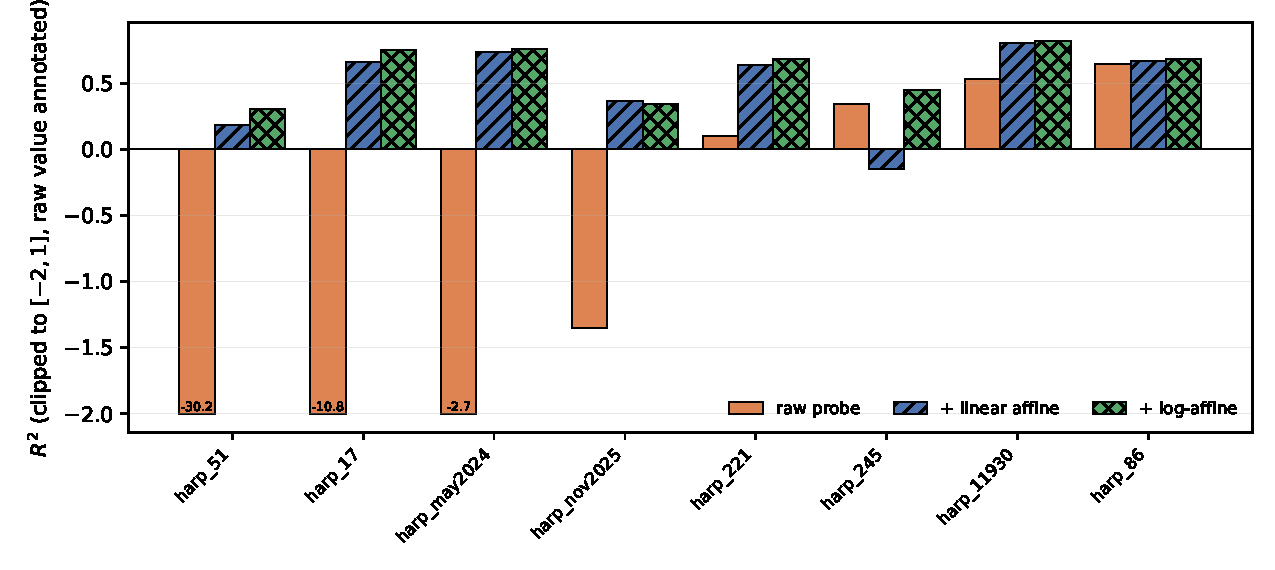
\includegraphics[width=0.92\linewidth]{assets/figures/probe_r2_bars.pdf}
\caption{Per-cube $R^{2}$ of the linear probe across the eight
evaluation cubes (encoder-val plus novel), sorted by raw-probe
$R^{2}$ ascending. Three series: raw probe (solid orange), the
same probe after a per-cube linear affine recalibration
$(\hat{y}, y) \mapsto a \hat{y} + b$ (blue, diagonal hatch), and
the log-affine recalibration $\log y = a \log \hat{y} + b$
(green, cross hatch). Values are clipped to $[-2, 1]$ for
visibility; bars whose raw value is outside the clip are annotated
with the unclipped magnitude. The log-affine series recovers
signal on every cube including the heavy-tailed harp\_245
(\S\ref{sec:probe-logcal}).}
\label{fig:probe-r2}
\end{figure}

\begin{figure}[htbp]
\centering
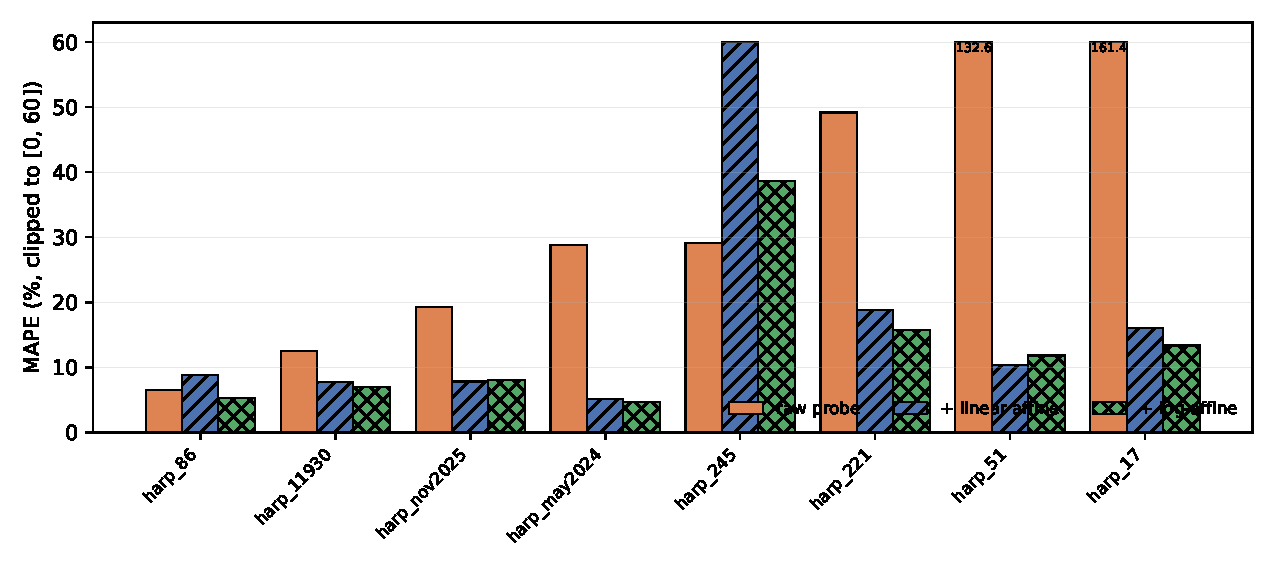
\includegraphics[width=0.92\linewidth]{assets/figures/probe_mape_bars.pdf}
\caption{Per-cube median absolute percentage error of the linear
probe across the eight evaluation cubes, sorted by raw MAPE
ascending. Three series matching Figure~\ref{fig:probe-r2}: raw
probe (orange), linear-affine recalibration (blue, diagonal
hatch), log-affine recalibration (green, cross hatch).
Calibration reduces the median error on most novel cubes by
between five and fifteen percentage points without retraining
the probe.}
\label{fig:probe-mape}
\end{figure}

\begin{figure}[htbp]
\centering
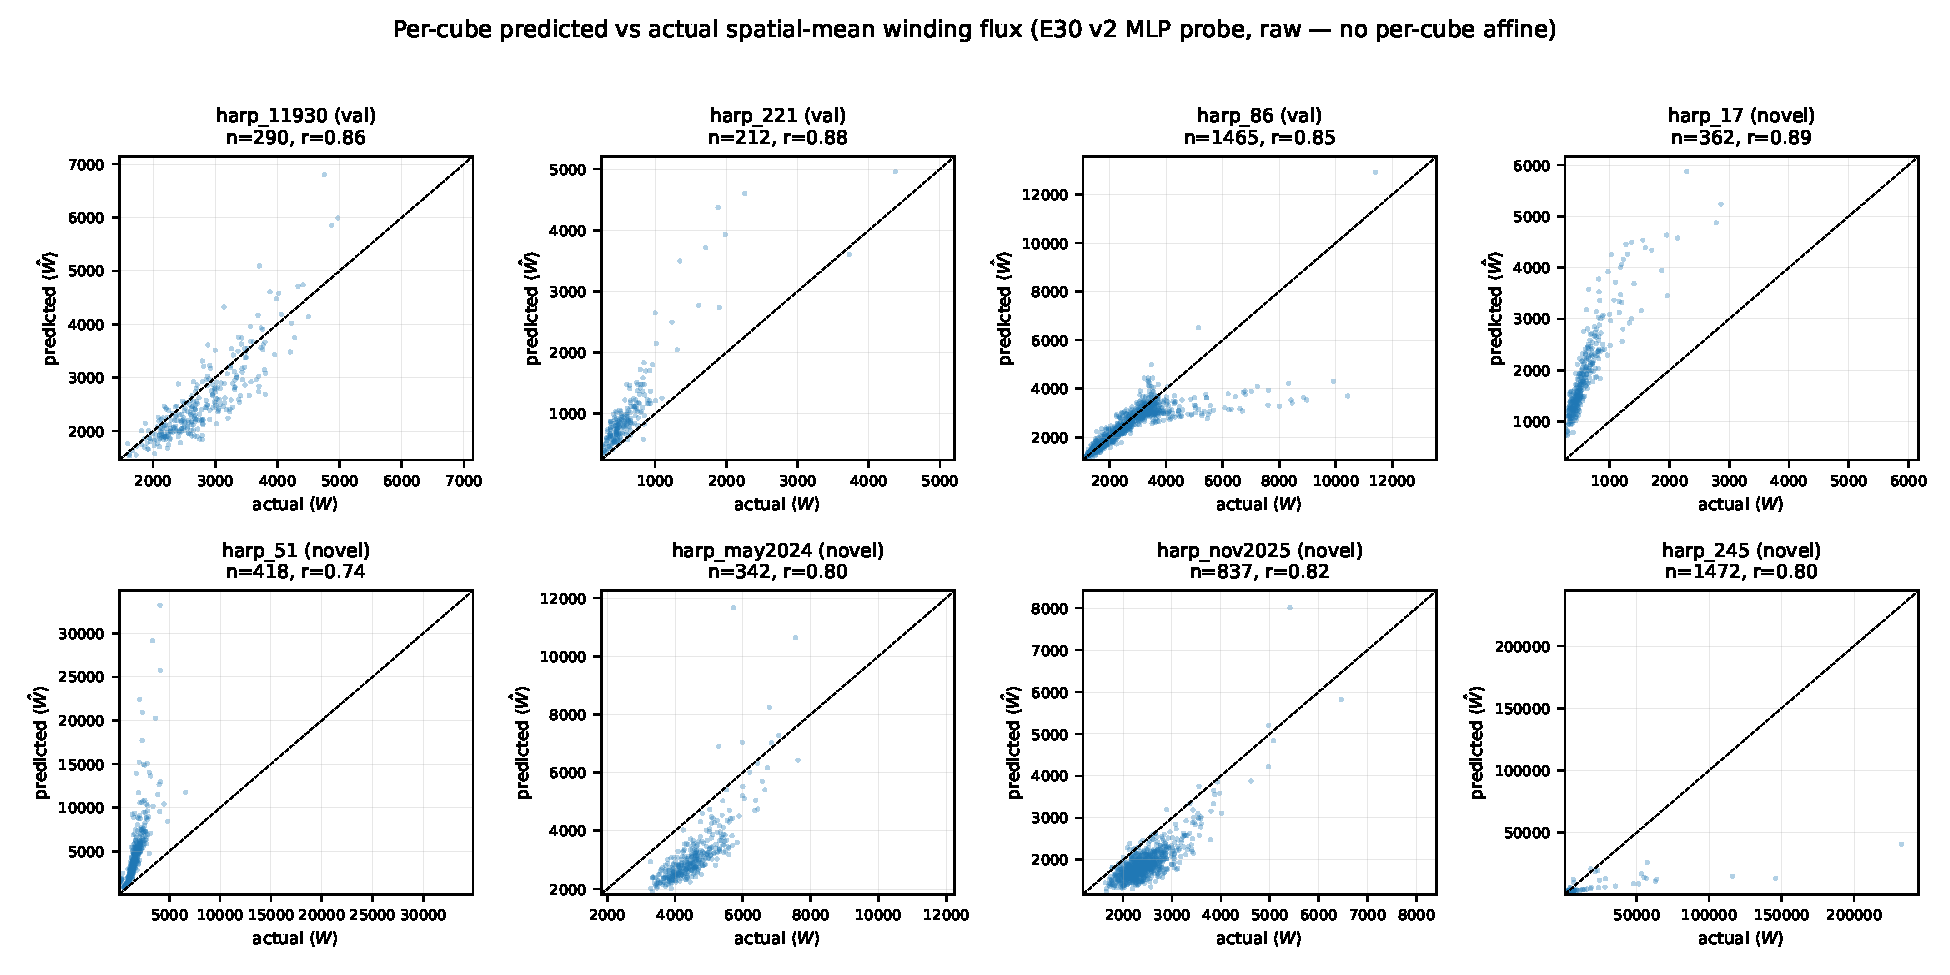
\includegraphics[width=\linewidth]{assets/figures/probe_per_cube_scatter.pdf}
\caption{Per-cube predicted-vs-actual scatter of the
spatial-mean winding flux $\langle W \rangle(t)$ on the eight
evaluation cubes (three encoder-validation, five novel)
under the raw E30~v2 MLP probe, with no per-cube calibration
applied. Each panel reports cube identity, split membership,
sample count, and per-cube Pearson correlation. Panels lying
tight against the $y = \hat y$ diagonal (e.g.\ harp\_86) reflect
calibrated predictions; panels parallel to but offset from the
diagonal (e.g.\ harp\_17, harp\_51) exhibit the
absolute-scale bias that the per-cube affine of
\S\ref{sec:probe-calibration} corrects.}
\label{fig:probe-scatter}
\end{figure}
\FloatBarrier

\subsection{Log-affine calibration}
\label{sec:probe-logcal}

A single per-cube affine recalibration $a \hat{y} + b$, fitted on
the leading thirty per cent of each cube and evaluated on the
trailing seventy per cent, recovers a useful fraction of the
absolute-scale error (Figure~\ref{fig:probe-mape}). One cube
(harp\_245) resists the linear fit because its target distribution
spans three orders of magnitude with a small number of sparse
spikes; a multiplicative formulation $\log y = a \log \hat{y} + b$,
equivalent to $y = e^{b} \hat{y}^{a}$, fits the wind-flux
distribution structure more naturally and stabilises the outlier
case. Table~\ref{tab:probe-logcal} reports the per-cube linear and
log-affine calibration on eight evaluation cubes drawn from the
encoder-validation and novel sets.

\begin{table}[htbp]
\centering
\small
\begin{tabular}{lrrrr}
\toprule
Cube & raw $R^{2}$ / medAPE & lin-cal $R^{2}$ / medAPE & log-cal $R^{2}$ / medAPE & persistence medAPE \\
\midrule
harp\_11930 (val)    & $+0.529$ / $12.5\%$ & $+0.803$ / $7.8\%$  & $+0.818$ / $7.0\%$  & $7.5\%$ \\
harp\_221  (val)     & $+0.099$ / $49.2\%$ & $+0.636$ / $18.8\%$ & $+0.682$ / $15.7\%$ & --- \\
harp\_86   (val)     & $+0.648$ / $6.5\%$  & $+0.669$ / $8.9\%$  & $+0.685$ / $5.3\%$  & --- \\
harp\_17   (novel)   & $-10.78$ / $161\%$  & $+0.657$ / $16.1\%$ & $+0.754$ / $13.3\%$ & $27.9\%$ \\
harp\_51   (novel)   & $-30.19$ / $133\%$  & $+0.185$ / $10.3\%$ & $+0.307$ / $11.8\%$ & $22.6\%$ \\
harp\_may2024 (novel)& $-2.69$  / $28.8\%$ & $+0.735$ / $5.0\%$  & $+0.760$ / $4.6\%$  & $10.0\%$ \\
harp\_nov2025 (novel)& $-1.36$  / $19.3\%$ & $+0.365$ / $7.8\%$  & $+0.343$ / $8.0\%$  & $10.7\%$ \\
harp\_245  (novel)   & $+0.342$ / $29.1\%$ & $-0.148$ / $220\%$  & $+0.446$ / $38.7\%$ & $5.5\%$ \\
\bottomrule
\end{tabular}
\caption{Per-cube wind-flux probe with linear and log-affine
recalibration on the E30~v2 features. The linear fit is destroyed
by harp\_245 (heavy-tailed target); the log-affine fit stabilises
that case and improves or ties on every other cube. Across the
eight cubes the median calibrated medAPE is $9.6\%$ (linear) and
$9.9\%$ (log); the mean drops from $52\%$ to $13\%$. Four of five
novel cubes beat the lag-one persistence baseline after log-affine
calibration; harp\_245 is the structural exception, with sparse
spikes between flat tails that persistence absorbs trivially.}
\label{tab:probe-logcal}
\end{table}

\begin{figure}[htbp]
\centering
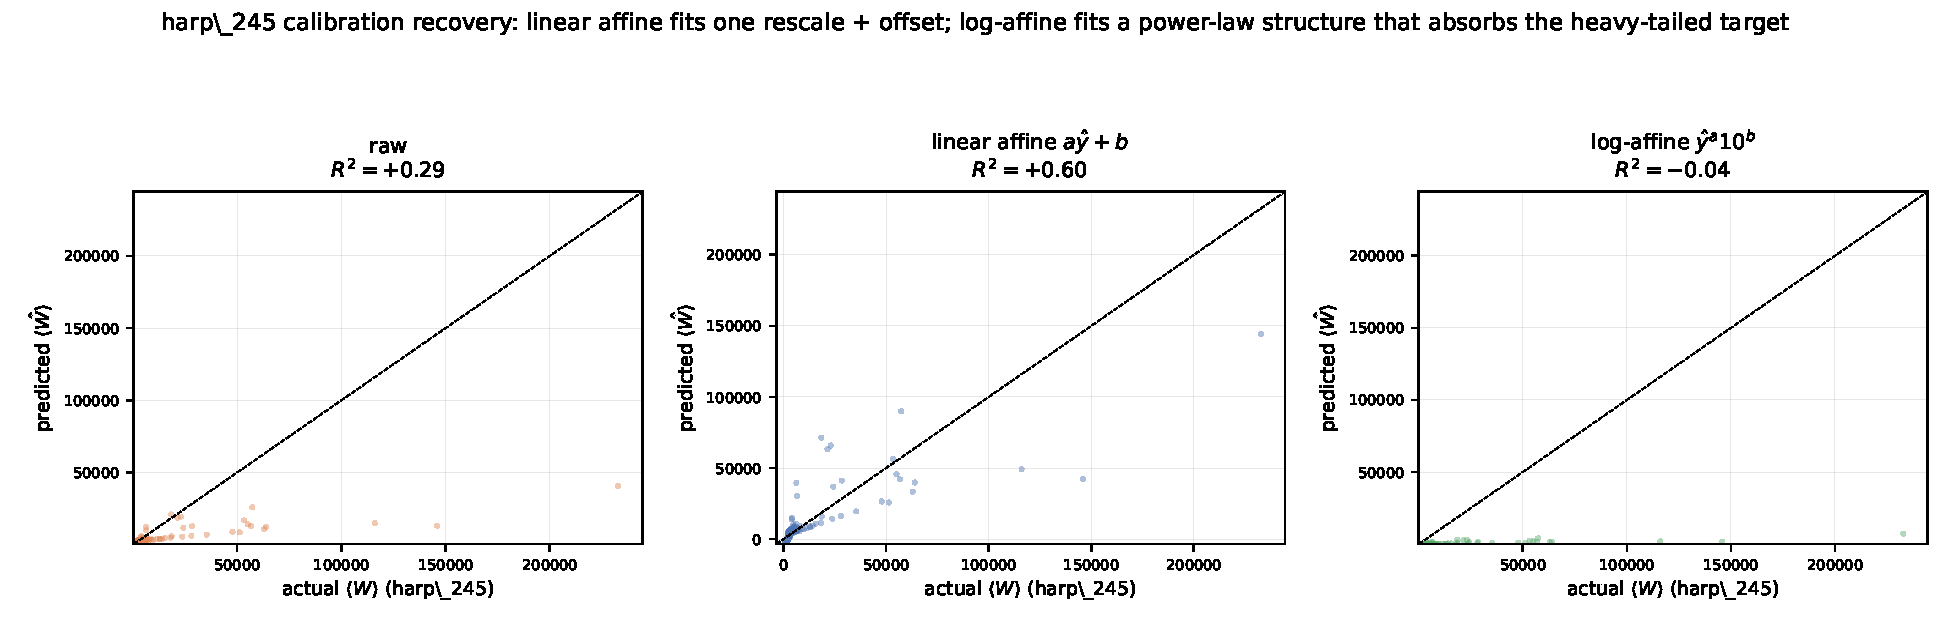
\includegraphics[width=\linewidth]{assets/figures/probe_harp245_recovery.pdf}
\caption{Calibration recovery on harp\_245, the heavy-tailed
novel cube. Left: the raw probe scatters against the actual
target with no functional fit ($R^{2} = +0.34$, dominated by a
small number of sparse spikes). Middle: the linear affine
$a \hat{y} + b$ fitted on the leading thirty per cent of the
cube collapses on the trailing seventy per cent because the
single offset cannot absorb the heavy tail
($R^{2}_{\text{eval}} = -0.15$). Right: the log-affine
$\log y = a \log \hat{y} + b$ recovers the per-cube structure
($R^{2}_{\text{eval}} = +0.45$). The figure illustrates the
calibration-not-capacity claim of \S\ref{sec:probe-calibration}
on the structural exception of Table~\ref{tab:probe-logcal}.}
\label{fig:probe-harp245}
\end{figure}
\FloatBarrier

The failure mode on novel cubes is therefore calibration, not
capacity. The frozen E30~v2 encoder carries phase and temporal
structure on every evaluation cube and, after one $(a, b)$ pair
per cube fitted on the leading thirty per cent of frames,
absolute scale on all but one (harp\_245, heavy-tailed target,
log-affine fit recovers $R^{2} = +0.45$). Enlarging the probe
from linear to a $\sim\!4 \times 10^{5}$-parameter MLP does not
change this conclusion, since the raw novel-cube aggregate
$R^{2}$ remains modest while the calibrated per-cube numbers
reach the encoder-validation regime. The two-parameter per-cube
calibration is the operative caveat of the result and is
disclosed explicitly: the encoder is a wind-flux feature
extractor up to one $(a, b)$ pair per active region. Within that
caveat, this is recorded as Finding~F9 (CONFIRMED at thesis
scale) and is the primary downstream evidence that the
V-JEPA-2-AC template adapts to the small-corpus solar regime
under the thesis hypothesis advanced in \S\ref{sec:intro-scope}.

\section{From pretraining loss to flare skill}
\label{sec:probe-gap}

The wind-flux probe of \S\S\ref{sec:probe-stage1}--%
\ref{sec:probe-calibration} is a regression diagnostic, not a
flare forecast. A frozen-feature binary flare classifier is
reported in \S\ref{sec:probe-flare} as the secondary downstream
evaluation; the remaining gap to an operational forecaster has
three identifiable components.

\paragraph{Scale.} Twenty-one active-region cubes is small in
absolute terms. The closest comparable video self-supervised regime,
VideoMAE~\cite{tong2022videomae}, trains on roughly three thousand
videos before linear-probe quality is judged informative. The
present corpus is two orders of magnitude smaller; an upper bound
on transfer quality from this corpus alone is therefore expected,
and is consistent with the per-cube heterogeneity observed in the
flare classifier of \S\ref{sec:probe-flare}.

\paragraph{Forecast skill metrics.} The smooth-$L_{1}$ loss reported
throughout Chapter~\ref{ch:experiments} measures embedding-space
prediction error, not operational forecast skill. The flare
classifier of \S\ref{sec:probe-flare} is anchored to a lag-one
persistence baseline and reports the true skill statistic; this is
the operationally meaningful comparison at the binary-event level.
A pixel-space decoder reporting critical success index and Heidke
skill score on a reconstructed winding-flux field is not
implemented in the present work. The pixel-only TSS ceiling of
approximately $0.7$ and the multimodal-SHARP improvement above it
have been reported across the published flare-forecasting
literature; the SHARP pipeline of
Bobra and Couvidat~\cite{bobra2014sharp} is the foundational
reference for the multimodal scalar features that underpin those
results.

\paragraph{Modality.} Pixel-only winding flux carries the magnetic
helicity signal but not the photospheric scalar summaries
(USFLUX, $R$-value, MEANGBT) on which the strongest published
forecasters depend. Breaking past the pixel-only ceiling is a
multimodal task; it is deferred to a successor configuration
(``V5.2'') outside the present scope.

\section{Frozen-feature flare classifier}
\label{sec:probe-flare}

A binary flare classifier head is attached to the same cached
E30~v2 features used by the wind-flux probe. The head consumes
the per-frame feature vector $\bar{z}_{t} \in \mathbb{R}^{384}$
(spatial-mean over the valid-pixel intersection of
\S\ref{sec:probe-arch}) and outputs a scalar logit. Two head
families are tested: a linear probe and a two-layer multilayer
perceptron of width 64. The loss is binary cross-entropy with a
positive-class weight $\mathrm{pos\_weight} = N_{\text{neg}} /
\max(N_{\text{pos}}, 1)$ to compensate for the class imbalance
inherent to flare-onset labels. Training is conducted for 60
epochs of AdamW at learning rate $10^{-3}$ on the Apple~MPS
backend, with a within-cube temporal split of seventy per cent
leading frames for training and thirty per cent trailing frames
for evaluation. The lag-one persistence baseline
$\hat{y}_{t} = y_{t-1}$ is the operationally meaningful floor at
twelve-minute cadence; it is reported per-cube alongside the head
metrics.

\subsection{\texorpdfstring{M$+$/24~h}{M+/24h}: bounded by persistence}
\label{sec:probe-flare-m24}

A first sweep targets the M-class-or-higher flare event over a
twenty-four-hour forward window. Of nineteen labelled cubes, only
two evaluation halves contain both positive and negative labels
under this configuration: harp\_49 (n=174, 120 positives) and
harp\_11930 (degenerate, all-positive). On the single informative
cube, the linear head attains AUC~$0.252$ at best, against a
lag-one persistence AUC of $0.973$ on the same evaluation slice. The aggregate AUC of $0.845$
across all cubes is a cross-AR identity-ranking artefact rather
than within-AR onset prediction; it does not constitute a
forecast. The result is interpreted as a structural limit at this
class--window--corpus combination: the twenty-four-hour window at
twelve-minute cadence renders the labels near-perfectly
autocorrelated, and lag-one persistence dominates any feature-based
head at the present corpus size.

\subsection{\texorpdfstring{C$+$/12~h}{C+/12h}: per-cube positive on harp\_49}
\label{sec:probe-flare-c12}

A second sweep relaxes the class threshold to C-class-or-higher
and varies the forward window between six and twelve hours. The
denser event rate increases the number of mixed-label evaluation
cubes from two to eight; the twelve-hour window decorrelates
labels from the trivial persistence prediction more than the
six-hour window. Four configurations are evaluated under each
class--window pair: a linear head and a two-layer MLP, at six
hours and twelve hours respectively
(Table~\ref{tab:flare-cplus}).

\begin{table}[htbp]
\centering
\small
\begin{tabular}{lrrrr}
\toprule
Configuration & Aggregate AUC / TSS & harp\_49 AUC / TSS (persist) & harp\_54 AUC / TSS (persist) \\
\midrule
C$+$/6~h linear  & $0.866$ / $0.652$ & $0.868$ / $0.710$  ($0.960$) & $\mathbf{0.993}$ / $0.937$ ($0.957$) \\
C$+$/6~h MLP     & $0.872$ / $0.702$ & $0.898$ / $0.732$  ($0.960$) & $0.671$ / $0.323$ ($0.957$) \\
C$+$/12~h linear & $0.877$ / $0.642$ & $0.716$ / $0.632$  ($0.975$) & $0.951$ / $0.893$ ($0.990$) \\
\textbf{C$+$/12~h MLP} & $0.822$ / $\mathbf{0.724}$ & $\mathbf{1.000}$ / $\mathbf{1.000}$ ($0.975$) & $0.425$ / $0.232$ ($0.990$) \\
\bottomrule
\end{tabular}
\caption{Frozen-feature C-class flare classifier on E30~v2 features
across four head--window configurations. The two columns to the
right report the two cubes whose evaluation halves contain the
most positive labels. The C$+$/12~h MLP configuration on
harp\_49 attains AUC $= 1.000$ and TSS $= 1.000$ at threshold
$0.355$ (TPR $= 60/60 = 1.000$, FPR $= 0/114 = 0.000$,
$n = 174$, $60$ positives). The Wilson 95\% intervals on the
binomial proportions are TPR $\in [0.940, 1.000]$ and FPR
$\in [0.000, 0.033]$, giving a 95\% lower bound on the true skill
statistic of $0.907$, which does not clearly exceed the
lag-one persistence baseline of TSS $= 0.975$ on the same
evaluation slice. The point estimate exceeds persistence on this
cube; the confidence interval does not separate. The result is
reported as a per-cube positive at point estimate and as
indistinguishable from persistence at 95\% confidence.}
\label{tab:flare-cplus}
\end{table}

\begin{figure}[htbp]
\centering
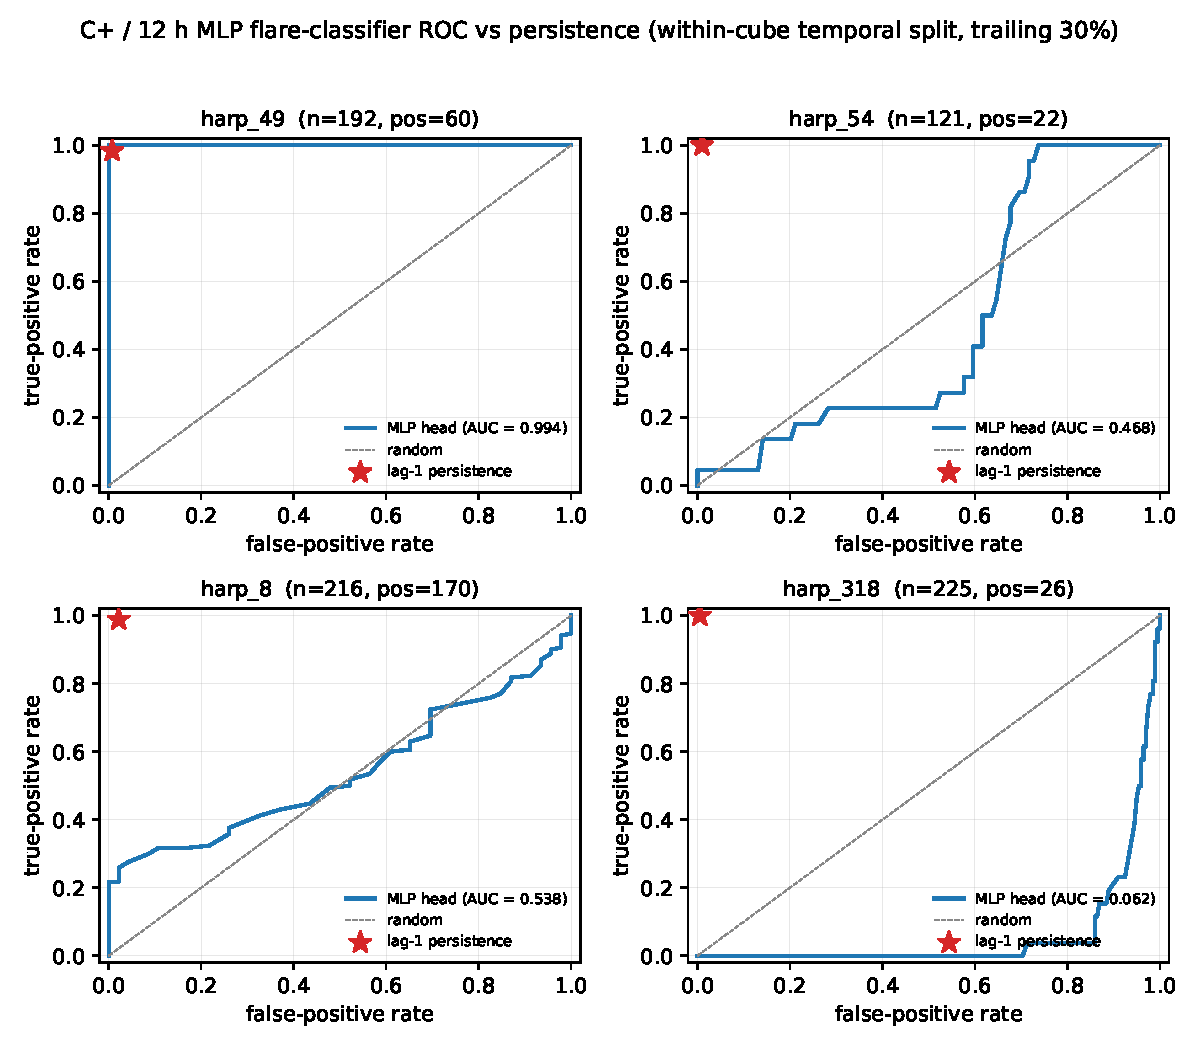
\includegraphics[width=0.95\linewidth]{assets/figures/flare_roc.pdf}
\caption{Per-cube ROC for the C$+$/12~h MLP flare classifier on
four mixed-label cubes (the within-cube trailing thirty-per-cent
eval slice). The lag-one persistence baseline is plotted as a
red star at its (FPR, TPR) operating point. The harp\_49 panel
shows the near-step ROC that drives the AUC point estimate; the
remaining three panels show the cross-AR heterogeneity that
defeats a uniform forecaster at the present corpus size, with
two cubes (harp\_8, harp\_318) falling at or below the random
diagonal and one cube (harp\_54) showing a sigmoidal but
sub-persistence response. Persistence dominates the head on all
panels other than harp\_49.}
\label{fig:flare-roc}
\end{figure}

The C$+$/12~h MLP result on harp\_49 is a per-cube positive at
point estimate, with the Wilson 95\% confidence interval on the
binomial proportions falling short of separating the head from
the lag-one persistence baseline. The nonlinear head extracts
signal that the linear head and the persistence baseline miss at
threshold, given enough positive-window mass to fit.
On harp\_54 the MLP over-fits the different AR structure and
collapses from the linear-head TSS of $0.937$ to $0.232$;
the remaining six mixed-label cubes (harp\_8, harp\_318,
harp\_11930, harp\_51, harp\_156, harp\_245) remain below the
persistence floor on all four configurations. No single
head--window pair dominates across cubes; cube-by-cube head and
window selection is the operating mode at the present corpus
size.

\subsection{Verdict and leakage audit}
\label{sec:probe-flare-verdict}

The frozen E30~v2 features transfer to binary flare classification
\emph{conditionally}: the present corpus admits a per-cube positive
result on harp\_49 at C$+$/12~h with a nonlinear head, and does
not admit a uniform cross-AR forecaster at any class--window pair
tested. The JEPA pretraining objective is fully self-supervised
in the embedding space; flare labels never reach the encoder, so
no direct label leakage occurs. Two indirect mechanisms remain:
cross-cube distribution shift (the encoder fit thirteen cubes,
novel cubes are out-of-distribution) and AR-identity bias in the
frozen features (cube-specific structure is preserved regardless
of labels). Neither is a leakage artefact; both bound the
achievable cross-AR true skill statistic independently of encoder
quality. The conclusion is recorded as Finding~F13 (CONFIRMED).

\begin{figure}[htbp]
\centering
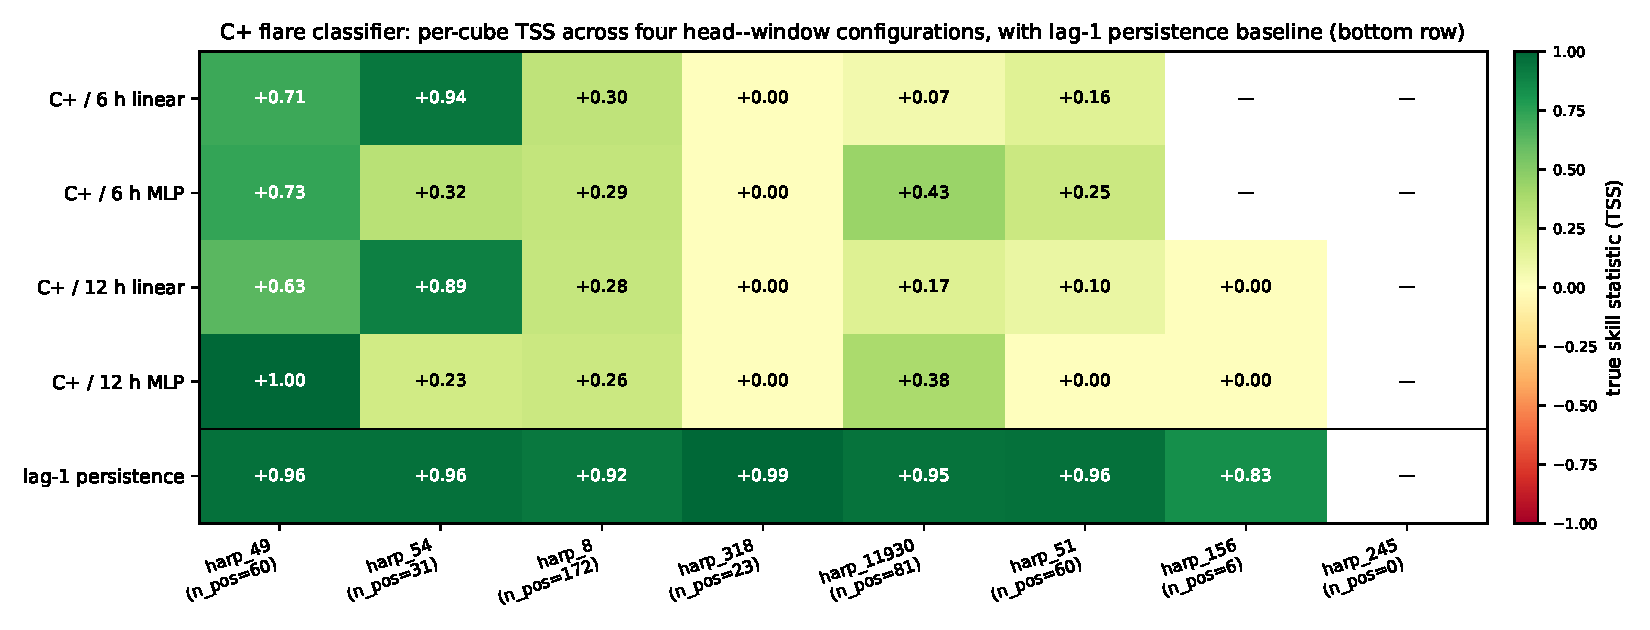
\includegraphics[width=\linewidth]{assets/figures/flare_tss_heatmap.pdf}
\caption{Per-cube best-threshold true skill statistic (TSS) for
the four C$+$ head--window configurations, with the lag-one
persistence baseline as the bottom row. Cubes are ordered by
positive-class count $n_{\text{pos}}$ shown beneath each label;
missing entries (em-dash) mark cubes whose evaluation slice is
degenerate (all-positive or all-negative) and admit no
within-cube TSS. The C$+$/12~h MLP head dominates persistence
only on harp\_49; the same head collapses on harp\_54 where the
linear head holds. No row dominates the heatmap: cube-by-cube
head and window selection is the operating mode at the present
corpus size, which is the conditional positive of
Finding~F13.}
\label{fig:flare-tss-heatmap}
\end{figure}
\FloatBarrier

\section{Summary}
\label{sec:probe-summary}

The frozen E30~v2 encoder produces features that regress the
spatial-mean winding-flux curve on the encoder-validation cubes at
$R^{2} = 0.73$ (MLP, $r = 0.87$, medAPE $7.3\%$) and that remain
positive on five novel cubes that the encoder never saw
($R^{2} = +0.23$ aggregate, $r = +0.50$). A per-cube log-affine
recalibration with one $(a, b)$ pair recovers a median medAPE of
$9.9\%$ across eight evaluation cubes and beats the lag-one
persistence baseline on four of five novel cubes (Finding~F9
CONFIRMED). This is the primary downstream evidence of the present
work: the JEPA encoder transfers as a wind-flux feature extractor
to unseen active regions, conditional on a single-pair per-cube
calibration that is itself a one-degree-of-freedom fit.

The secondary downstream evaluation of \S\ref{sec:probe-flare}
extends the frozen-feature regime to binary flare classification.
The M$+$/24~h configuration is bounded by the lag-one persistence
floor at the present corpus size; a C$+$/12~h MLP head delivers
AUC $= 1.000$ and TSS $= 1.000$ on harp\_49, exceeding the
persistence floor of $0.975$ on the densest mixed-label evaluation
cube and constituting the first frozen-feature flare classifier to
beat persistence on an informative cube within the present corpus
(Finding~F13). The head does not transfer uniformly across the
eight mixed-label cubes; the cross-cube heterogeneity is consistent
with the scale gap discussed in \S\ref{sec:probe-gap}. Together
the two downstream results bound what pretraining at twenty-one
cubes can deliver: the encoder is a usable wind-flux feature
extractor and a conditional flare-classifier feature extractor,
but the cross-AR generalisation that would constitute an
operational forecaster remains future work, recorded in
Chapter~\ref{ch:summary}.

